% \section{Preliminaries}

As the name suggests, quantum graphs model quantum mechanical particles on graph-like objects, edges joined in vertices. From a physical point of view, a quantum graph can be considered to be a network of thin (approximately one-dimensional) conductive wires on which quantum mechanical phenomena occur. On the graph, an electric and/or magnetic potential may be present. The main objective is to study how quantum mechanical particles---it is natural to consider electrons---propagate through the graph. The study of quantum graphs originated in 1930s as models for free electrons in molecules, and materials such as graphene have been modeled by quantum graphs.

% Note that we are not restricted to only quantum mechanics, in the sense that any wave-like phenomena described by sine and cosine functions or complex exponentials, such as waves in a fluid, can be modeled by the eigenfunctions of $L u = \lambda u$, where $L = - \Dopn{x}{2}$ and $\lambda$ represents the energy or frequency of the wave.

% Quantum graphs are studied both for their purely mathematical properties, and also because they are models for certain physical systems. Typical examples are systems that can be approximated as thin one-dimensional networks on which quantum mechanical phenomena occur. Indeed, quantum graphs originated as models for free electrons in molecules, and materials such as graphene have been modeled by quantum graphs.

Mathematically quantum graphs are defined as metric graphs, where edges are joined at vertices, along with a differential operator acting on functions defined on the metric graph. Most commonly one studies the eigenvalue problem of the magnetic Schrödinger operator
\[
  L_{q,a} = \g{i\Dop{x}+a(x)}^2+q(x).
\]
That is, one solves the time-independent Schrödinger equation
\[
  L_{q,a} \psi = \lambda \psi
\]
for a quantum mechanical particle living on the graph, where an electric potential $q(x)$ and magnetic potential $a(x)$ is applied. A metric graph is depicted in \cref{fig: basic quantum graph}.

\begin{figure}[h]
 \centering
  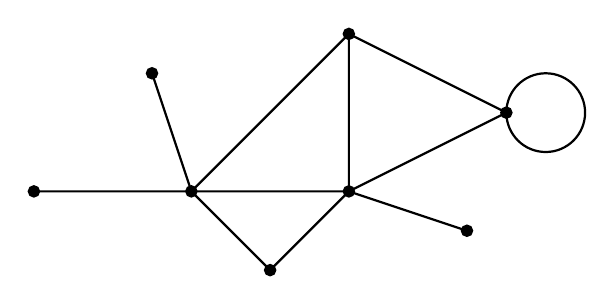
\begin{tikzpicture}[vertex/.style={draw,circle,minimum size=1.3mm,inner sep=0pt,outer sep=0pt,fill=black},scale=2, line width=0.8pt]
    \coordinate (p1) at (0,0);
    \coordinate (p2) at (1,0);
    \coordinate (p3) at (2,0);
    \coordinate (p4) at (2,1);
    \coordinate (p5) at (1.5,-0.5);
    \coordinate (p6) at (3,0.5);
    \coordinate (p7) at (2.75,-0.25);
    \coordinate (p8) at (0.75,0.75);
    % \coordinate (p9) at (3.5,0.5);
    \draw (p1)--(p2)--(p3)--(p4)--(p6);
    \draw (p2)--(p4);
    \draw (p3)--(p5);
    \draw (p2)--(p5);
    \draw (p3)--(p6);
    \draw (p3)--(p7);
    \draw (p2)--(p8);
    \draw (3.25,0.5) circle (0.25);
    \node[vertex] at (p1) {};
    \node[vertex] at (p2) {};
    \node[vertex] at (p3) {};
    \node[vertex] at (p4) {};
    \node[vertex] at (p5) {};
    \node[vertex] at (p6) {};
    \node[vertex] at (p7) {};
    \node[vertex] at (p8) {};
    % \node[vertex] at (p9) {};
  \end{tikzpicture}
  \caption{A graph.}
  \label{fig: basic quantum graph}
\end{figure}


For the equation to represent a physical system with real energies $\lambda$ one requires the operator $L_{q,a}$ to be self-adjoint. In particular this puts constraints on what can happen at the vertices, we must have certain matching conditions. The standard matching condition requires the functions to be continuous at every vertex, and in addition the sum of the outgoing derivatives from a vertex must be zero. This gives that the quantum probability of the wave is preserved after propagation through a vertex.

The purpose of this chapter is to bridge the gap between the point of view of readers more familiar with either mathematics or physics. We will introduce the aspects of quantum mechanics relevant for the study of quantum graphs and translate from the language of quantum mechanics to that of quantum graphs. More advanced concepts are deferred to the subsequent sections. In \cref{sec: defining quantum graphs} we properly define quantum graphs and further discuss metric graphs, differential operators, self-adjointness and matching conditions. In \cref{sec: properties} we explore various properties of quantum graphs and give several examples. All this builds up to \cref{sec: snowflake} where we introduce the snowflake graph, the central object of this thesis.

The quantum snowflake is defined as an infinite radial quantum tree graph that is also self-similar. By radial we mean that all properties of the graph, such as edge lengths and matching conditions, depend only on the distance from the root of the tree. The graph is self-similar in the sense that if one picks a vertex and cuts off the part of the graph that contains the root vertex, the remaining infinite subgraph is structurally identical to the original graph. In particular we require the length of every edge $e$ to be given by $\ell\beta^n$ where $n$ is the number of edges between $e$ and the root vertex, for $0<\beta<1$ we get a graph with finite depth $\ell/(1-\beta)$. On the graph we shall have standard matching conditions and no potentials.

The main objective will be to study the scattering properties of the quantum snowflake. Scattering phenomena is discussed in a more general context in \cref{sec: properties} and should be thought of as describing what information one can get out of a graph by physically examining it. To ``look'' at any object, in particular one described by a quantum graph, one shoots radiation, such as electrons, towards the object and observes how it scatters from the object. That is, we will characterize reflection and absorption for waves of varying energies that are sent into the snowflake graph.

We shall study the rotational symmetry of the snowflake graph, from which it will be possible to represent all eigenfunctions on the graph as a sum of quasi rotation invariant functions. This will allow us to collapse all edges in one generation into only one edge, from which the function values on all other edges can be reconstructed. Using this together with the self-similarity of the graph we can reduce the entire snowflake graph to a line graph with special snowflake matching conditions.

On the resulting line graph we shall further reduce the complexity by combining all vertices into one meta-vertex. This will lead to a recursive expression for the scattering coefficient for the general snowflake of $n$ generations.

This reduction of the graph greatly simplifies the study of the quantum snowflake and gives a better understanding of the internal scattering. It will be shown how the total scattering emerges from reflections on each edge of the graph.

As we will see, the general structure of the scattering from the snowflake graph is highly irregular. For the special case when the graph is periodic, i.e.\ all edges are of equal length, much more can be said. We shall show that the periodic snowflake gives rise to a band gap structure, similar to that of crystalline materials. This phenomena should be understood as arising from the fact that there exist energies that are not realizable inside the graph, therefore giving total reflection.

Finally the thesis is concluded with \cref{sec: conclusion} where we discuss of the obtained results and give indications for possible improvements and further research.




% \section{Physical interpretation}

% One should keep in mind that the mathematical models and assumptions ultimately stem from observations of nature, and can in principle not be derived mathematically. Oh really? Think about the Mathematical Universe Hypothesis.



\section{The Schrödinger equation}

It is well known that the Schrödinger equation describes the motion and behavior of quantum mechanical particles. The Schrödinger equation is often stated to be the result of empirical observations and therefore not possible to derive mathematically. However, one can arrive at the Schrödinger equation by starting from classical mechanics and imposing certain correspondence rules. In this section we motivate the Schrödinger equation by assuming that matter particles possess wave-like properties. By matter particle we mean the particles of which ordinary matter consists of, more specifically one may talk about fermions, the points is to distinguish from photons which we already know possesses wave-like properties. A more elaborate derivation of the Schrödinger equation starting from electromagnetic waves can be found in \cite{SE derivaiton}. There are indeed many ways to approach quantum mechanics and the Schrödinger equation, for instance quantization of classical mechanics or Feynman's path integral formulation, cf.\ \cite{feynman quantum mechanics}.

The following is a very naive derivation of the Schrödinger equation, illustrating how the equation arises from adding a wave-like property to classical particles, inspired by that of photons.

Let us consider a classical particle with mass $m$ and momentum $p$, the total energy is then $E = T + V$ where $T = \frac{p^2}{2m}$ is the kinetic energy and $V$ is the potential energy (from, say, an electric field) which we can leave unspecified, i.e.
\begin{equation}\label{eq: total energy}
  E = \frac{p^2}{2m} + V.
\end{equation}

We now introduce de Broglie's hypothesis, namely that matter particles possess wave-like properties just like photons. For photons we have the Planck--Einstein relation
\begin{equation}\label{eq: planck-einstein relation}
  E = h\nu
\end{equation}
relating the total energy $E$ to the frequency $\nu$ of the electromagnetic wave, where $h$ is Planck's constant. Furthermore, the energy--momentum relation states that
\begin{equation}\label{eq: energy-momentum relation}
  E^2 = (pc)^2 + (mc^2)^2
\end{equation}
for any particle, where $m$ is the intrinsic rest mass of the particle. Photons have no rest mass so this reduces to $E = pc$, where the velocity $c$ is given by $\lambda \nu$, where $\lambda$ is the wavelength. Using this we can combine the relations \eqref{eq: planck-einstein relation} and \eqref{eq: energy-momentum relation} to get
\begin{equation}\label{eq: de broglie relation}
  E = h \nu = pc = p \lambda \nu \iff p = \frac{h}{\lambda}.
\end{equation}
De Broglie's insight was that the wave-like property (which we are now introducing) of matter particles also obeys this relation, namely $p = h/\lambda$. The wavelength $\lambda$ is then interpreted as the wavelength of the matter wave associated with the particle, described by its wave function $\psi$. With no additional restrictions on the wave function it would take the general form of d'Alembert waves
\[ \psi(x, t) = f(x - vt) + g(x + vt) \]
but we will for now consider the case of simple plane waves
\[ \psi(x, t) = Ae^{i(kx - \omega t)} + Be^{i(-kx - \omega t)}. \]
(Plane waves corresponds to freely propagating waves, we will see more on this in section~\ref{sec: stationary states}.)
The wave number $k$ is related to the wavelength $\lambda$ by $k = \frac{2\pi}{\lambda}$. Using the de Broglie relation \eqref{eq: de broglie relation} we then have
\begin{equation}\label{eq: k-p relation}
  k = \frac{p}{\hbar}
\end{equation}
where $\hbar = \frac{h}{2\pi}$ is the reduced Planck constant.
Differentiating $\psi$ with respect to the spatial coordinate gives
\[ \pD{\psi}{x}(x, t) = ik\psi(x, y) = i\frac{p}{\hbar} \psi(x, t), \]
hence we have the momentum operator relation
\[ p = -i\hbar\pDop{x}. \]
We only see that this holds for plane waves $\psi(x, t) = Ae^{i(kx - \omega t)} + Be^{i(-kx - \omega t)}$, but this is indeed a general result.
Now, we can write equation \eqref{eq: total energy} as
\begin{equation}\label{eq: tise}
  E \psi = -\frac{\hbar^2}{2m}\pDn{\psi}{x}{2} + V\psi.
\end{equation}
We have arrived at the time-independent Schrödinger equation, TISE.

Furthermore, if we relate $E$ to the temporal frequency $\frac{\omega}{2\pi}$ of the wave function via the Planck--Einstein relation \eqref{eq: planck-einstein relation}---which we can use since we have assumed a wave-like property matter particles similar to that of photons---we have
\[ E = \hbar \omega. \]
Differentiating $\psi$ with respect to the temporal coordinate, and using the above relation, gives
\[ \pD{\psi}{t}(x,t) = -iw\psi(x,t) = \frac{-iE}{\hbar} \psi(x,t), \]
that is
\begin{equation}
  E\psi(x,t) = i \hbar \pD{\psi}{t}(x,t).
\end{equation}
Substituting this for the left hand side in the time-independent Schrödinger equation \eqref{eq: tise} gives
\begin{equation}\label{eq: tdse}
  i \hbar \pD{\psi}{t} = -\frac{\hbar^2}{2m}\pDn{\psi}{x}{2} + V\psi,
\end{equation}
the time-dependent Schrödinger equation, TDSE.

In our example we can introduce the Hamiltonian $H$ as the operator defined by the expression
\[ H = \widehat{T} + \widehat{V} = -\frac{\hbar^2}{2m}\pDopn{x}{2} + V(x) \]
where
\[ \widehat{T} = -\frac{\hbar^2}{2m}\pDopn{x}{2} = \frac{\widehat{p}^2}{2m} \]
is identified as the kinetic energy operator with
\[ \widehat{p} = -i \hbar \pDop{x} \]
being the momentum operator and $\widehat{V} = V(x)$ is the potential energy operator. The TDSE can then be written more compactly as
\[ i\hbar \pD{\psi}{t} = H\psi \]
and the TISE becomes an eigenvalue equation for the operator $H$
\[ H\psi = E\psi. \]
The Hamiltonian recovered above is the usual Hamiltonian for a particle propagating under the influence of a potential $V(x)$, but for other particular systems the Hamiltonian may take another form.
If we use natural units where $\hbar=1$ and let the $m = 1/2$, so that $\frac{\hbar^2}{2m} = 1$, and denote the energy in these normalized units by $\lambda$, then the TISE for the usual Hamiltonian can be written as
\[ L_q\psi = \lambda\psi. \]
That is $H = L_q$ where $L_q$ was defined in \eqref{eq: magnetic schrödinger operator}. The magnetic potential is taken into account by letting
\[ \widehat{p} = -i \pDop{x} - a(x), \]
then $H = L_{q,a}$. In the subsequent sections we will only use normalized units, as described above.



\section{Quantum states and interpretations of quantum mechanics}\label{sec: quantum states and interpretations of quantum mechanics}

Classically, properties of an object, or the \emph{state} of an object, is characterized by its position and momentum. In quantum mechanics the state of a particle is instead specified by its wave function, containing information about both the position and momentum of the particle. The Schrödinger equation gives the possible such states, their corresponding energies, and how they evolve over time.

A fundamental property of quantum mechanics is that quantities such as energy for a particle can be constrained to discrete values, for example the energy of an electron bound to an atom. However, a freely propagating electron can take energies from a continuous spectrum. Recall from section~\ref{sec: spectrum} that the spectrum of linear operators may have this property, namely the spectrum can be both discrete and continuous. It is therefore a postulate of quantum mechanics that to each dynamical variable, ``observable'', there corresponds a linear operator such that all possible values of the variable are given by the spectrum of the operator.

The \emph{ground state energy} (zero-point energy) is the lowest positive eigenvalue $\lambda_0$, the higher eigenvalues are called excited state energies.

% For many graphs also $\lambda = 0$ is an eigenvalue, however this energy is not physically realizable because of the uncertainty principle. As can be shown, the wave function $\psi(x)$ in position space and wave function $\widetilde{\psi}(p)$ in momentum space are Fourier transform duals of each other. Hence we have $\sigma_x\sigma_p \le 1$, where $\sigma_a$ denotes the standard deviation of a variable $a$, (the lower bound depends on which particular definition of the Fourier transform that is being used, and what units we assume). From this we see that $E=0$ is not possible, since this is implies zero kinetic energy, i.e.\ zero momentum, hence $E>0$.

The statistical interpretation of quantum mechanics, introduced by Max Born in \cite{born statistical interpretation}, originally motivated entirely by observation, states that the probability of observing a quantum mechanical particle at a particular location $x$ and time $t$ is given by the probability density function $\abs{\psi(x,t)}^2$, this fact is known as the Born rule.
% This also exemplifies why one requires $\psi \in L^2$, so that the total probability equals unity.

Although this thesis primarily deals with the mathematical properties of quantum graphs, we will broaden our view of the physical significance of the mathematics and highlight questions that arise when interpreting the models by making a slight detour into the interpretation of quantum mechanics, by discussing the so called measurement problem.

Quantum mechanical particles are often spread out in space, in the sense that $\psi(x)$ is non-zero on some interval (in fact, time evolution tends to smear out the wave function), while on the other hand, a measurement of the position of a particle always yields a specific position, in accordance with the Born rule. The wave-like property can only be implicitly detected by studying interference of the wave function.
% In the context of quantum graphs, the stationary states of any graph have a wave function that is non-zero almost everywhere on the entire graph, while any attempt to measure the position of the particle will yield a specific position.

This seemingly collapse of the wave function, from being smeared out to becoming highly localized, is not in any way described by the mathematics of quantum mechanics. The text-book approach of describing this is by adding a postulate to the model, namely that the wave function collapses (i.e.\ becomes highly localized) to the measured value. This is what is known as the Copenhagen interpretation. This interpretation arguably has several issues, for example, what precisely constitutes a measurement? Any interaction of particles is in a sense a measurement. Einstein's objection is often quoted as ``God does not throw dice'', pointing out that the random collapse of the wave function is ill-justified and not consistent with our otherwise deterministic model of reality. Other so called collapse theories exist, perhaps most noteworthy is the Ghirardi--Rimini--Weber theory, postulating that the wave function undergoes spontaneous collapse and random yet very frequent points in time. This avoids the problem of what denotes a measurement in the Copenhagen interpretation while still giving predictions that are in agreement with observations.

Any collapse theory will necessarily contain fundamental randomness. This may seem unavoidable if the Born rule is to be satisfied, but this is not the case. The mathematically simplest interpretation is to not add any additional postulates, contrary to the other interpretations, that is to say that the wave function never collapses, it continues to evolve deterministically according to the Schrödinger equation. In this interpretation every measurement entangles the ``observer'' to the measured system, thus entering a superposition state. Measurements are then not distinguished from any other form of interaction between particles, unlike in the Copenhagen interpretation.

This entails that the entire environment gets entangled to the quantum state being measured, from which the classical state emerges as an apparent collapse of the wave function, an effect called decoherence. In this interpretation every possible classical state exists in a superposition. This gives rise to the Many Worlds Interpretation originally introduced by Hugh Everett, in which, by the effect of decoherence, non-interacting branches of the wave-function (and in extension reality) get created. The Born rule is then an emerging property in every decohered slice of reality \cite{carroll EQM probability, wallace born rule}.

One may argue that the interpretation is not important, since all interpretations give equal predictions, but this is not necessarily the case. There are contrived gedanken experiments for which, for example, collapse theories and the many world theory gives different predictions \cite{vaidman mwi}.

A radically different approach is Quantum Bayesianism, in which one assumes that quantum states do not represent elements of physical reality \cite{qbism introduction, qbism and the greeks}. This is a rather pragmatic approach in which quantum mechanics is merely a tool for making statistical predictions, in this way avoiding the problematic implications of interpreting quantum states as representations of physical reality.

Towards the other extreme we have the Mathematical Universe Hypothesis by Max Tegmark \cite{tegmark}, essentially extending from the Many worlds interpretation, postulating that the physical world is an abstract mathematical structure. Hence stating that quantum states truly are elements of physical reality (provided that quantum mechanics is a correct description of reality).

There is no consensus on how quantum mechanics is to be interpreted, and the discussion quickly becomes philosophical. There is however no doubt in that it is a very successful theory in the sense that all predictions so far are in perfect agreement with empirical results.
% In what follows we will generally not be concerned with interpretations and when necessary we will apply the Born rule without further ado.



\section{Stationary states}\label{sec: stationary states}

Stationary states are states that do not evolve over time, in the sense that $\abs{\psi(x,t)}^2$ is constant in $t$, stationary. This allows for a time dependence of the probability amplitude $\psi(x,t)$ only as a phase shift $e^{i\theta(t)}$, where $\theta(t) \in \R$. As we will see in equation \ref{eq: time-separated solution}, the phase is given by $\theta(t) = -\lambda t$. Stationary states are important since they are the states of equilibrium, states reached after some time when the system has settled.
% The study of quantum graphs mainly focuses on such states.
% General solutions to the Schrödinger equation can be expressed as a series of stationary states, therefore most attention is directed towards stationary states.
Considering only stationary states greatly simplifies matters, since the TISE is an ordinary differential equation while the TDSE is a partial differential equations. On the other hand, every solution to the TDSE can be written as a superposition of stationary states, showing that it is essentially sufficient to consider such states.

The stationary solutions to the time-dependent Schrödinger equation \eqref{eq: tdse} can be found by using separation of variables with the Ansatz
\[ \psi(x,t) = u(x) T(t). \]
This then gives, with $q(x) \equiv a(x) \equiv 0$ for convenience,
\[
  i \Dop{t} u(x) T(t) = - \Dopn{x}{2} u(x) T(t) \iff
  i \frac{\D{T}{t}(t)}{T(t)} = - \frac{\Dn{u}{x}{2}(x)}{u(x)} = \lambda,
\]
for some constant $\lambda$. That is,
\begin{align*}
  i \D{T}{t}(t) &= \lambda T(t) \\
  - \Dopn{x}{2}u(x) &= \lambda u(x).
\end{align*}
The second equation is precisely the time-independent Schrödinger equation for the spatial component $u(x)$, justifying that the constant $\lambda$ is to be interpreted as the energy of the system (in normalized units). With $k^2 = \lambda$ we can write the solutions for $u(x)$ as
\[ u(x) = Ae^{ikx} + Be^{-ikx} \]
and the solution for the time component $T(t)$ as
\begin{equation}\label{eq: time-separated solution}
  T(t) = e^{-i\lambda t}.
\end{equation}
Hence the solution to the TDSE is given by
\begin{equation}\label{eq: left right waves}
  \psi(x,t) = Ae^{i(kx-\lambda t)} + Be^{i(-kx-\lambda t)},
\end{equation}
showing that the two terms can be interpreted as right and left traveling waves, respectively. The constants $A$ and $B$ and possible values of $\lambda$ are to be determined by the particular situation, see for instance example~\ref{ex: particle in a box}.

The wave function of a stationary state is given by standing waves, evolving in time only by changing the phase shift.

The criteria of $H$ being self-adjoint, discussed in \ref{sec: differential operators}, is important in the quantum mechanical interpretation. It ensure that the model is physical in the sense that the eigenvalues of $H$ are real, which is necessary since this represents the energy of the system. Furthermore, the eigenvectors of $H$ are then orthogonal and can be chosen so that they form an orthonormal basis of the state space. This, together with the linearity of the equation, allows any solution of the TDSE to be written as a linear combination of stationary states, showing that it is sufficient, without loss of generality, to consider only the stationary states.


